\section{Back propagation in CNN - Convolution in each direction!}

In this question, we are going to do back propagation for a Convolutional layer and come up with a closed form answer for our required derivatives. First, let's look at the general schema of our layer:

\begin{center}
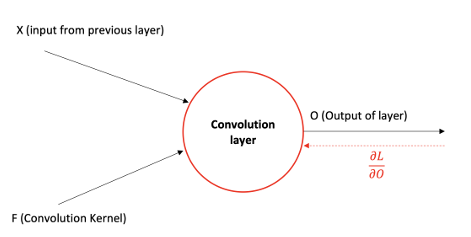
\includegraphics[width = 0.8\textwidth]{convolution_layer_diagram.png} % Save your diagram image as convolution_layer_diagram.png in the same directory as this .tex file.
\end{center}

We know how \textbf{Forward Pass} for convolution layers are computed (if not, please refer to the course's slides!). Suppose \( X \) is a 2D matrix and thus, \( F \) is also 2D. Please note that the dimensions of these 2 matrices can arbitrarily change. Prove that:

$$\frac{\partial L}{\partial F} = X * \frac{\partial L}{\partial O}$$
$$\frac{\partial L}{\partial X} = F \circledast \frac{\partial L}{\partial O}$$

where \( * \) sign is Convolution operation and \( \circledast \) is full convolution.

It is worth noting that \( * \) sign is Convolution operation and \( \circledast \) is full convolution.
\begin{qsolve}
    \begin{qsolve}[]
        first lets prove the first statement(\( \frac{\partial L}{\partial F} = X * \frac{\partial L}{\partial O} \)):

        we know that $O_{i,j} = \sum_{m=0}^{M-1} \sum_{n=0}^{N-1} X_{i+m,j+n} F_{m,n}$ and $L = \sum_{i=0}^{I-1} \sum_{j=0}^{J-1} L_{i,j}$ so we can write:
        
        \begin{center}
            \hl{$ \frac{\partial L}{\partial F_{m,n}} = \sum_{i=0}^{I-1} \sum_{j=0}^{J-1} \frac{\partial L}{\partial O_{i,j}} \frac{\partial O_{i,j}}{\partial F_{m,n}} = \sum_{i=0}^{I-1} \sum_{j=0}^{J-1} \frac{\partial L}{\partial O_{i,j}} X_{i+m,j+n}$}       
        \end{center}
        
        the above equation is the same as the convolution operation so we can write:
        $$ \frac{\partial L}{\partial F} = X * \frac{\partial L}{\partial O}$$
        \splitqsolve[\splitqsolve]
        now lets prove the second statement(\( \frac{\partial L}{\partial X} = F \circledast \frac{\partial L}{\partial O} \)):
        we can rewrite $\frac{\partial L}{\partial X_{i,j}}$ as below:

        \begin{center}
            \hl{$ \frac{\partial L}{\partial X_{i,j}} = \sum_{m=0}^{M-1} \sum_{n=0}^{N-1} \frac{\partial L}{\partial O_{i-m,j-n}} F_{m,n}$}
        \end{center}

        the right side of the above equation comes from the fact that $O_{i-m , j-n} = \sum_{m=0}^{M-1} \sum_{n=0}^{N-1} X_{i,j} F_{m,n}$ so $\frac{\partial O_{i-m,j-n}}{\partial X_{i,j}} = F_{m,n}$.

        the above equation is the same as the full convolution operation so we can write:
        $$ \frac{\partial L}{\partial X} = F \circledast \frac{\partial L}{\partial O}$$
    \end{qsolve}
\end{qsolve}
